\documentclass[11pt]{article}

\usepackage{fancyhdr}
\usepackage{amsmath}
\usepackage{tikz}
\usepackage{pgfplots}
\pgfplotsset{compat=1.18}

\pagestyle{fancy}
\fancyhead[L]{AP Calculus BC}
\fancyhead[R]{1.5 Functions and Logarithms}
\fancyfoot[C]{\thepage}

\newcommand{\emptygraph}{
    \begin{center}
    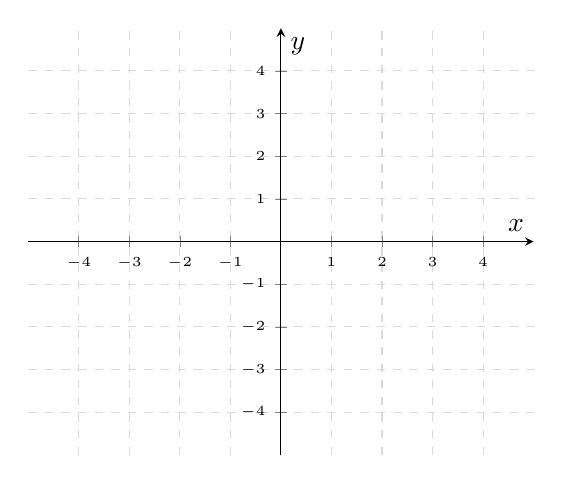
\begin{tikzpicture}
        \begin{axis}[
            axis lines = middle,
            grid = both,
            width=8cm,
            height=7cm,
            xmin=-5, xmax=5,
            ymin=-5, ymax=5,
            xtick={-4,-3,...,4},
            ytick={-4,-3,...,4},
            xlabel={$x$},
            ylabel={$y$},
            tick label style={font=\tiny},
            grid style={dashed, gray!30}
        ]
        \end{axis}
    \end{tikzpicture}
    \end{center}
}

\begin{document}

\noindent What is a function?

\vspace{1.5cm}

\noindent What is a one-to-one function?

\noindent Definition: a function $f(x)$ is one-to-one on domain $D$ if $f(a) \neq f(b)$ whenever $a \neq b$ (note that we can make a function one-to-one by \underline{\hspace{2cm}}).

\noindent This leads to a question: who cares?

\vspace{1.5cm}

\noindent An inverse means that we took the $x$ and $x$ (or $f(x)$) and flipped them. Find the inverse of $y = f(x) = -2 + 4$.

\vspace{1.5cm}

\noindent Graph the function and its inverse. What is $(f \circ g)(x)$?

\emptygraph

\noindent Do all of that again for $f(x) = x^2, x > 0$. This time do it parametrically.

\emptygraph

\noindent What is the inverse of $y=a^x (a > 0, a \neq 1)$? (Why the limitations?)

\vspace{1.5cm}

\noindent What is the domain and rang of \underline{\hspace{3cm}}? Graph:

\emptygraph

\noindent Quick refresher: write the inverse of $y = \log_2 x$ and $y = 3^x$

\vspace{1.5cm}

\noindent What do we call $y = \ln x$? What is the base? What about $y = \log x$?

\vspace{1.5cm}

\noindent Refresh on log properties:
\noindent Solve for x:


\begin{align*}
    \ln x = 3t + 5 && e^{2x} = 10
\end{align*}

\noindent Properties / Rules of logarithms:

\begin{itemize}
    \item Product: $\log_b m \times n = \log_b m + log_b n$
    \item Quotient: $\log_b \frac{m}{n} = \log_b m - log_b n$
    \item Power: $\log_bm^p = p \times \log_b m$
\end{itemize}

\noindent How about the change of base formula? Use it to graph $f(x) = \log_2 x$.

\emptygraph

\noindent Application: Sarah invest \$$1000$ in an account that earns $5.25$\% interest compounded annually. How long will it take the account to get to \$$2500$?

\end{document}
